\documentclass[tikz,border=12pt]{standalone}
\usepackage[T1]{fontenc}
\usepackage{tgheros}
\usepackage{sfmath}
\usepackage{amsmath}
\usepackage{tikz}
\usetikzlibrary{arrows.meta,positioning,shapes.geometric,fit,backgrounds,calc,patterns}
\usepackage{xcolor}

\renewcommand{\familydefault}{\sfdefault}

% Harvard Crimson & ETH Zurich Academic Semantic Palette
\definecolor{harvardcrimson}{HTML}{A51C30}
\definecolor{ethdarkblue}{HTML}{1F407A}
\definecolor{ethblue}{HTML}{215CAF}
\definecolor{ethpetrol}{HTML}{007A87}
\definecolor{ethbronze}{HTML}{B87333}
\definecolor{ethpurple}{HTML}{5B4B8A}
\definecolor{ethslate}{HTML}{475569}
\definecolor{darkslate}{HTML}{0F172A}
\definecolor{cardbg}{HTML}{FFFFFF}
\definecolor{subtlebg}{HTML}{F8FAFC}
\definecolor{cardborder}{HTML}{CBD5E1}
\definecolor{alertred}{HTML}{DC2626}
\definecolor{amberalert}{HTML}{D97706}
\definecolor{softgreen}{HTML}{059669}

\begin{document}
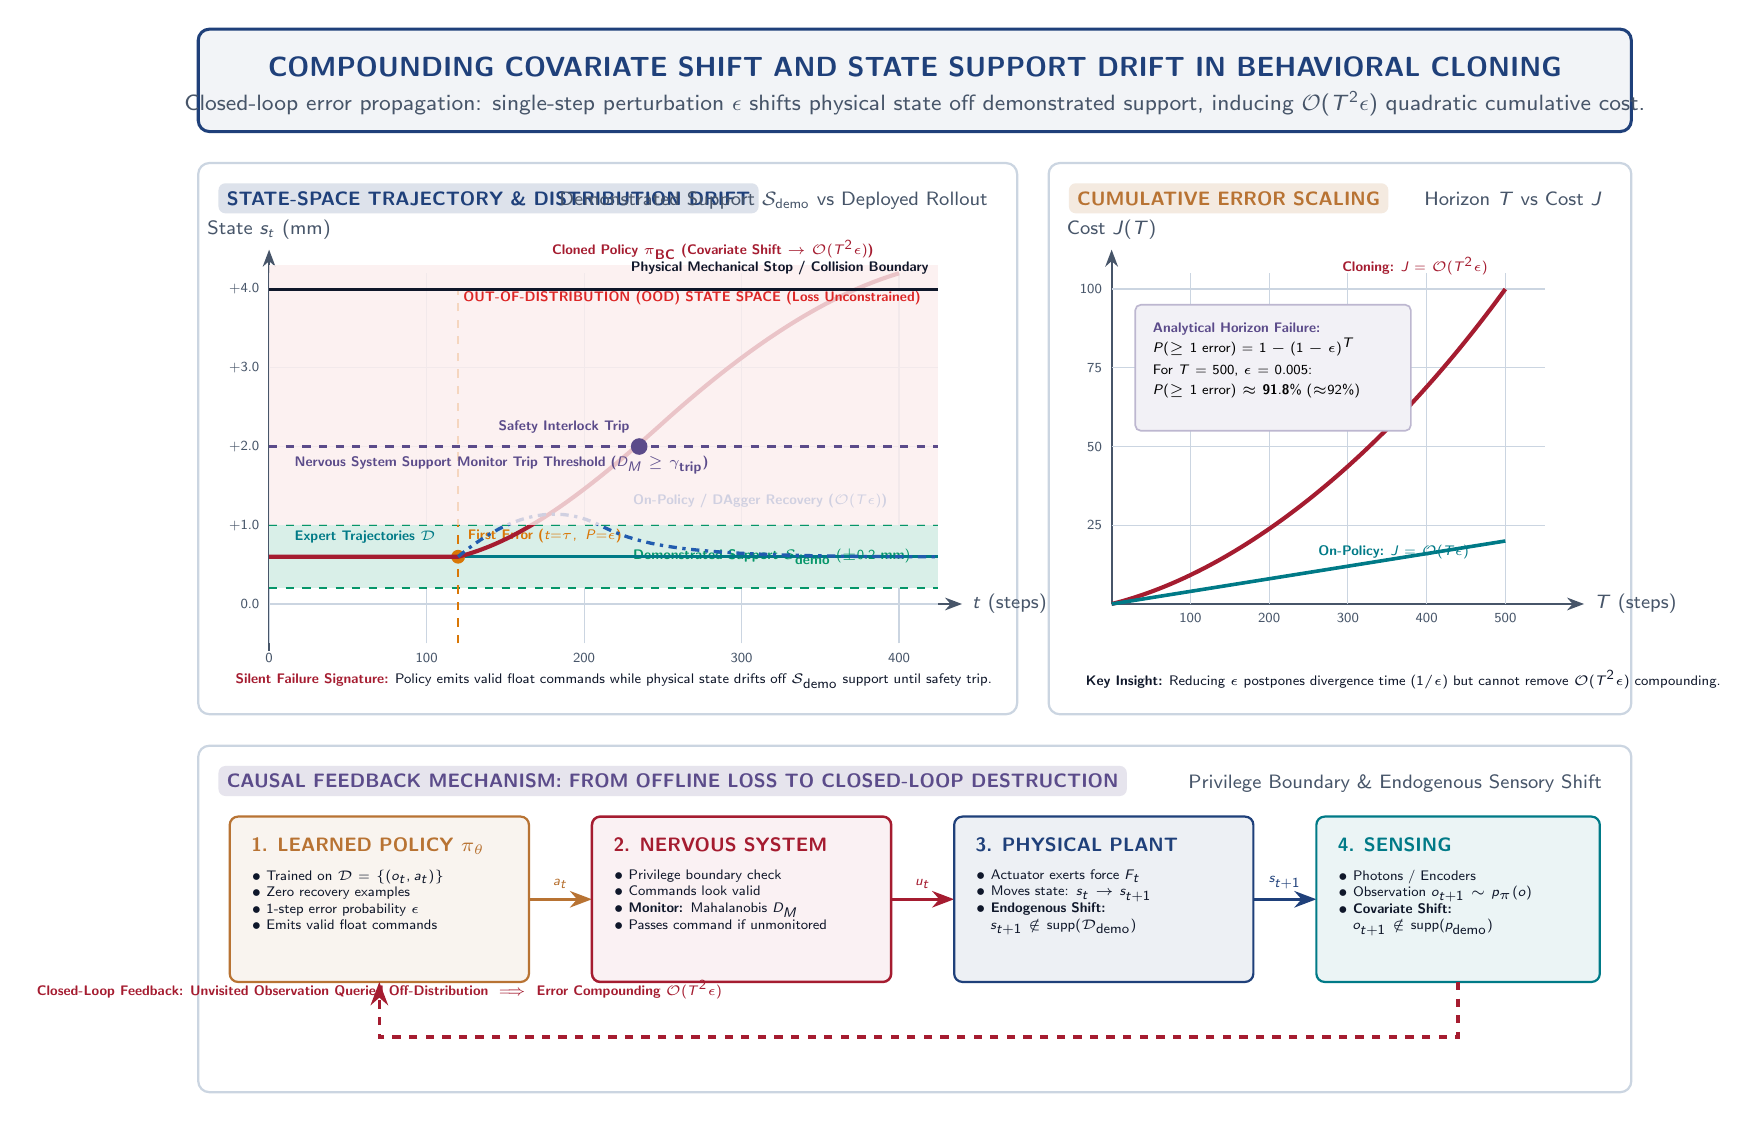
\begin{tikzpicture}[
  font=\sffamily,
  >=Stealth,
  panelbg/.style={
    draw=cardborder,
    fill=cardbg,
    rounded corners=4pt,
    line width=0.8pt
  },
  headerpill/.style={
    font=\sffamily\bfseries\scriptsize,
    rounded corners=2.5pt,
    inner sep=3pt
  },
  infobox/.style={
    rounded corners=2.5pt,
    font=\tiny,
    inner sep=3.5pt,
    line width=0.6pt
  }
]

  % =========================================================================
  % TOP HEADER BANNER
  % =========================================================================
  \draw[draw=ethdarkblue, fill=ethdarkblue!6, rounded corners=4pt, line width=1.1pt] (0, 12.2) rectangle (18.2, 13.5);
  \node[font=\normalsize\bfseries\color{ethdarkblue}, anchor=center] at (9.1, 13.02) {COMPOUNDING COVARIATE SHIFT AND STATE SUPPORT DRIFT IN BEHAVIORAL CLONING};
  \node[font=\footnotesize\color{ethslate}, anchor=center] at (9.1, 12.55) {Closed-loop error propagation: single-step perturbation $\epsilon$ shifts physical state off demonstrated support, inducing $\mathcal{O}(T^2 \epsilon)$ quadratic cumulative cost.};

  % =========================================================================
  % PANEL A: STATE-SPACE TRAJECTORY & SUPPORT MANIFOLD
  % =========================================================================
  \begin{scope}[shift={(0, 4.8)}]
    \draw[panelbg] (0, 0) rectangle (10.4, 7.0);

    % Header Pill
    \node[headerpill, fill=ethdarkblue!15, text=ethdarkblue, anchor=north west] at (0.25, 6.75) {STATE-SPACE TRAJECTORY \& DISTRIBUTION DRIFT};
    \node[font=\scriptsize\color{ethslate}, anchor=north east] at (10.15, 6.75) {Demonstrated Support $\mathcal{S}_{\text{demo}}$ vs Deployed Rollout};

    % Coordinate Frame inside Panel A
    \begin{scope}[shift={(0.9, 1.4)}]
      % Axes: Time t vs State Displacement x(t)
      \draw[->, line width=0.7pt, color=ethslate] (0, 0) -- (8.8, 0) node[right, font=\scriptsize] {$t\ (\text{steps})$};
      \draw[->, line width=0.7pt, color=ethslate] (0, -0.6) -- (0, 4.5) node[above, font=\scriptsize] {State $s_t\ (\text{mm})$};

      % Ticks
      \foreach \x/\label in {0/0, 2.0/100, 4.0/200, 6.0/300, 8.0/400} {
        \draw[color=cardborder, line width=0.4pt] (\x, -0.5) -- (\x, 4.2);
        \node[font=\tiny\color{ethslate}, below] at (\x, -0.5) {\label};
      }
      \foreach \y/\label in {0/0.0, 1.0/+1.0, 2.0/+2.0, 3.0/+3.0, 4.0/+4.0} {
        \draw[color=cardborder, line width=0.4pt] (0, \y) -- (8.5, \y);
        \node[font=\tiny\color{ethslate}, left] at (0, \y) {\label};
      }

      % Demonstrated State Support Tube (Shaded Green/Petrol: +/- 0.2 mm around y=0.5)
      \fill[softgreen!15] (0, 0.2) -- (8.5, 0.2) -- (8.5, 1.0) -- (0, 1.0) -- cycle;
      \draw[softgreen, dashed, line width=0.7pt] (0, 0.2) -- (8.5, 0.2);
      \draw[softgreen, dashed, line width=0.7pt] (0, 1.0) -- (8.5, 1.0);
      \node[font=\tiny\bfseries\color{softgreen}, anchor=west] at (4.5, 0.6) {Demonstrated Support $\mathcal{S}_{\text{demo}}\ (\pm 0.2\text{ mm})$};

      % Nominal Expert Demonstration Trajectory (y = 0.6)
      \draw[line width=1.2pt, color=ethpetrol] (0, 0.6) -- (8.5, 0.6);
      \node[font=\tiny\bfseries\color{ethpetrol}, anchor=south west] at (0.2, 0.65) {Expert Trajectories $\mathcal{D}$};

      % First Error Perturbation at t = tau (tau = 120 steps -> x = 2.4)
      \draw[dashed, line width=0.8pt, color=amberalert] (2.4, -0.5) -- (2.4, 4.0);
      \fill[amberalert] (2.4, 0.6) circle (2.5pt);
      \node[font=\tiny\bfseries\color{amberalert}, above right] at (2.4, 0.65) {First Error ($t{=}\tau,\ P{=}\epsilon$)};

      % Deployed Behavioral Cloning Policy (Diverging OOD Trajectory)
      \draw[line width=1.5pt, color=harvardcrimson] 
        (0, 0.6) -- (2.4, 0.6) 
        .. controls (3.2, 0.8) and (4.0, 1.4) .. (5.0, 2.3)
        .. controls (6.0, 3.2) and (7.0, 3.9) .. (8.0, 4.2);
      \node[font=\tiny\bfseries\color{harvardcrimson}, anchor=south east] at (7.8, 4.25) {Cloned Policy $\pi_{\text{BC}}$ (Covariate Shift $\to \mathcal{O}(T^2\epsilon)$)};

      % Recovery-Trained / DAgger Trajectory (Corrects back into tube)
      \draw[line width=1.2pt, color=ethblue, dashdotted]
        (2.4, 0.6) 
        .. controls (3.0, 1.1) and (3.6, 1.3) .. (4.2, 1.0)
        .. controls (4.8, 0.7) and (5.4, 0.6) .. (8.5, 0.6);
      \node[font=\tiny\bfseries\color{ethblue}, anchor=south west] at (4.5, 1.1) {On-Policy / DAgger Recovery ($\mathcal{O}(T\epsilon)$)};

      % Out-of-Distribution Shaded Zone
      \fill[alertred!8, opacity=0.8] (0, 1.0) rectangle (8.5, 4.3);
      \node[font=\tiny\bfseries\color{alertred}, anchor=north east] at (8.4, 4.1) {OUT-OF-DISTRIBUTION (OOD) STATE SPACE (Loss Unconstrained)};

      % Runtime Detector Trip Line (Mahalanobis Threshold at y=2.0 / x=4.7)
      \draw[dashed, line width=0.9pt, color=ethpurple] (0, 2.0) -- (8.5, 2.0);
      \node[font=\tiny\bfseries\color{ethpurple}, anchor=north west] at (0.2, 2.0) {Nervous System Support Monitor Trip Threshold ($D_M \ge \gamma_{\text{trip}}$)};
      \fill[ethpurple] (4.7, 2.0) circle (3pt);
      \node[font=\tiny\bfseries\color{ethpurple}, above left] at (4.7, 2.05) {Safety Interlock Trip};

      % Hard Mechanical Stop / Collision Boundary (y = 4.0)
      \draw[line width=1.1pt, color=darkslate] (0, 4.0) -- (8.5, 4.0);
      \node[font=\tiny\bfseries\color{darkslate}, anchor=south east] at (8.5, 4.05) {Physical Mechanical Stop / Collision Boundary};
    \end{scope}

    % Bottom Diagnostic Note
    \node[font=\tiny\color{darkslate}, anchor=south west] at (0.35, 0.2) {
      \textbf{\color{harvardcrimson}Silent Failure Signature:} Policy emits valid float commands while physical state drifts off $\mathcal{S}_{\text{demo}}$ support until safety trip.
    };
  \end{scope}

  % =========================================================================
  % PANEL B: CUMULATIVE COST BOUND COMPARISON (O(T^2 epsilon) vs O(T epsilon))
  % =========================================================================
  \begin{scope}[shift={(10.8, 4.8)}]
    \draw[panelbg] (0, 0) rectangle (7.4, 7.0);

    % Header Pill
    \node[headerpill, fill=ethbronze!15, text=ethbronze, anchor=north west] at (0.25, 6.75) {CUMULATIVE ERROR SCALING};
    \node[font=\scriptsize\color{ethslate}, anchor=north east] at (7.15, 6.75) {Horizon $T$ vs Cost $J$};

    % Coordinate Frame inside Panel B
    \begin{scope}[shift={(0.8, 1.4)}]
      % Axes
      \draw[->, line width=0.7pt, color=ethslate] (0, 0) -- (6.0, 0) node[right, font=\scriptsize] {$T\ (\text{steps})$};
      \draw[->, line width=0.7pt, color=ethslate] (0, 0) -- (0, 4.5) node[above, font=\scriptsize] {Cost $J(T)$};

      % Ticks
      \foreach \x/\label in {1.0/100, 2.0/200, 3.0/300, 4.0/400, 5.0/500} {
        \draw[color=cardborder, line width=0.4pt] (\x, 0) -- (\x, 4.2);
        \node[font=\tiny\color{ethslate}, below] at (\x, 0) {\label};
      }
      \foreach \y/\label in {1.0/25, 2.0/50, 3.0/75, 4.0/100} {
        \draw[color=cardborder, line width=0.4pt] (0, \y) -- (5.5, \y);
        \node[font=\tiny\color{ethslate}, left] at (0, \y) {\label};
      }

      % Quadratic Compounding Curve: J = epsilon * T*(T+1)/2 (Crimson)
      % For epsilon=0.0008: T=500 -> J = 100 -> y=4.0
      \draw[line width=1.5pt, color=harvardcrimson]
        (0, 0) .. controls (1.6, 0.4) and (3.4, 1.8) .. (5.0, 4.0);
      \node[font=\tiny\bfseries\color{harvardcrimson}, anchor=south east] at (4.9, 4.05) {Cloning: $J = \mathcal{O}(T^2 \epsilon)$};

      % Linear On-Policy Curve: J = c * T * epsilon (Petrol)
      \draw[line width=1.3pt, color=ethpetrol] (0, 0) -- (5.0, 0.8);
      \node[font=\tiny\bfseries\color{ethpetrol}, anchor=south west] at (2.5, 0.45) {On-Policy: $J = \mathcal{O}(T \epsilon)$};

      % Statistical Error Probability Callout Box
      \draw[fill=ethpurple!8, draw=ethpurple!40, rounded corners=2pt, line width=0.6pt] (0.3, 2.2) rectangle (3.8, 3.8);
      \node[anchor=north west, font=\tiny, text width=3.3cm] at (0.4, 3.7) {
        \textbf{\color{ethpurple}Analytical Horizon Failure:}\\
        $P(\ge 1\text{ error}) = 1 - (1 - \epsilon)^T$\\[2pt]
        For $T = 500$, $\epsilon = 0.005$:\\[1pt]
        $P(\ge 1\text{ error}) \approx \mathbf{91.8\%}$ (${\approx}92\%$)
      };
    \end{scope}

    % Bottom Note
    \node[font=\tiny\color{darkslate}, anchor=south west] at (0.35, 0.2) {
      \textbf{\color{darkslate}Key Insight:} Reducing $\epsilon$ postpones divergence time ($1/\epsilon$) but cannot remove $\mathcal{O}(T^2\epsilon)$ compounding.
    };
  \end{scope}

  % =========================================================================
  % PANEL C: THE CLOSED-LOOP CAUSAL CHAIN OF COVARIATE SHIFT
  % =========================================================================
  \begin{scope}[shift={(0, 0)}]
    \draw[panelbg] (0, 0) rectangle (18.2, 4.4);

    % Header Pill
    \node[headerpill, fill=ethpurple!15, text=ethpurple, anchor=north west] at (0.25, 4.15) {CAUSAL FEEDBACK MECHANISM: FROM OFFLINE LOSS TO CLOSED-LOOP DESTRUCTION};
    \node[font=\scriptsize\color{ethslate}, anchor=north east] at (17.95, 4.15) {Privilege Boundary \& Endogenous Sensory Shift};

    % Step 1 Box: Policy Network
    \draw[draw=ethbronze, fill=ethbronze!8, rounded corners=3pt, line width=0.8pt] (0.4, 1.4) rectangle (4.2, 3.5);
    \node[font=\scriptsize\bfseries\color{ethbronze}, anchor=north west] at (0.55, 3.35) {1. LEARNED POLICY $\pi_\theta$};
    \node[font=\tiny\color{darkslate}, anchor=north west, text width=3.4cm] at (0.55, 2.95) {
      $\bullet$ Trained on $\mathcal{D} = \{(o_t, a_t)\}$\\
      $\bullet$ Zero recovery examples\\
      $\bullet$ 1-step error probability $\epsilon$\\
      $\bullet$ Emits valid float commands
    };

    % Arrow 1 -> 2
    \draw[->, line width=1.1pt, color=ethbronze] (4.2, 2.45) -- (5.0, 2.45)
      node[midway, above, font=\tiny\bfseries\color{ethbronze}] {$a_t$};

    % Step 2 Box: Privilege Boundary & Nervous System
    \draw[draw=harvardcrimson, fill=harvardcrimson!6, rounded corners=3pt, line width=0.9pt] (5.0, 1.4) rectangle (8.8, 3.5);
    \node[font=\scriptsize\bfseries\color{harvardcrimson}, anchor=north west] at (5.15, 3.35) {2. NERVOUS SYSTEM};
    \node[font=\tiny\color{darkslate}, anchor=north west, text width=3.4cm] at (5.15, 2.95) {
      $\bullet$ Privilege boundary check\\
      $\bullet$ Commands look valid\\
      $\bullet$ \textbf{Monitor:} Mahalanobis $D_M$\\
      $\bullet$ Passes command if unmonitored
    };

    % Arrow 2 -> 3
    \draw[->, line width=1.1pt, color=harvardcrimson] (8.8, 2.45) -- (9.6, 2.45)
      node[midway, above, font=\tiny\bfseries\color{harvardcrimson}] {$u_t$};

    % Step 3 Box: Physical Plant & Actuator
    \draw[draw=ethdarkblue, fill=ethdarkblue!8, rounded corners=3pt, line width=0.8pt] (9.6, 1.4) rectangle (13.4, 3.5);
    \node[font=\scriptsize\bfseries\color{ethdarkblue}, anchor=north west] at (9.75, 3.35) {3. PHYSICAL PLANT};
    \node[font=\tiny\color{darkslate}, anchor=north west, text width=3.4cm] at (9.75, 2.95) {
      $\bullet$ Actuator exerts force $F_t$\\
      $\bullet$ Moves state: $s_t \to s_{t+1}$\\
      $\bullet$ \textbf{Endogenous Shift:}\\
      $\quad s_{t+1} \notin \text{supp}(\mathcal{D}_{\text{demo}})$
    };

    % Arrow 3 -> 4
    \draw[->, line width=1.1pt, color=ethdarkblue] (13.4, 2.45) -- (14.2, 2.45)
      node[midway, above, font=\tiny\bfseries\color{ethdarkblue}] {$s_{t+1}$};

    % Step 4 Box: Sensor Transduction
    \draw[draw=ethpetrol, fill=ethpetrol!8, rounded corners=3pt, line width=0.8pt] (14.2, 1.4) rectangle (17.8, 3.5);
    \node[font=\scriptsize\bfseries\color{ethpetrol}, anchor=north west] at (14.35, 3.35) {4. SENSING};
    \node[font=\tiny\color{darkslate}, anchor=north west, text width=3.2cm] at (14.35, 2.95) {
      $\bullet$ Photons / Encoders\\
      $\bullet$ Observation $o_{t+1} \sim p_\pi(o)$\\
      $\bullet$ \textbf{Covariate Shift:}\\
      $\quad o_{t+1} \notin \text{supp}(p_{\text{demo}})$
    };

    % Closed-loop feedback return arrow: 4 -> 1
    \draw[->, line width=1.2pt, color=harvardcrimson, dashed] 
      (16.0, 1.4) -- (16.0, 0.7) -- (2.3, 0.7) -- (2.3, 1.4)
      node[pos=0.5, above, font=\tiny\bfseries\color{harvardcrimson}] {Closed-Loop Feedback: Unvisited Observation Queried Off-Distribution $\implies$ Error Compounding $\mathcal{O}(T^2\epsilon)$};

  \end{scope}

\end{tikzpicture}
\end{document}